%%%%%%%%%%%%%%%%%%%%%%%%%%%%%%%%%%%%%%%%%%%%%%%%%%%
% DECLARATION DE LA CLASSE DU DOCUMENT
%%%%%%%%%%%%%%%%%%%%%%%%%%%%%%%%%%%%%%%%%%%%%%%%%%%
%% Utiliser le format suivant:
% \documentclass[type de papier% ("letterpaper" demandé)
% , simple ou recto verso% ("oneside" ou "twoside")%
% , taille de la police% ("12pt" demandé)%
% , type de document% ("these", "memoire" ou "thesepararticles")%
% , langue du document ("francais" ou "english")%
% , options supplémentaires% ("creativecommons" pour préciser que le document est soumis à la licence créative commomns, "hyperref", "withAlgo2e" pour utiliser le package algorithm2e avec la mise en page correcte de la liste des algorithmes)
%]{thETS}

%% Exemple pour une thèse creative commons, utilisant le package hyperref
\documentclass[letterpaper
, twoside
, 12pt
,these
,francais
,creativecommons,hyperref
]{thETS}

\usepackage[utf8]{inputenc}
\usepackage{glossaries}
\usepackage{todonotes}

\makeindex
\makeglossaries
\newacronym{HOL}{HOL}{Higher Order Logic}

\usepackage{float}
\floatstyle{boxed}
\restylefloat{figure}

%%%%%%%%%%%%%%%%%%%%%%%%%%%%%%%%%%%%%%%%%%%%%%%%%%%
% IMPORTANT: NOTES D'IMPRESSION POUR RESPECTER LES MARGES
%%%%%%%%%%%%%%%%%%%%%%%%%%%%%%%%%%%%%%%%%%%%%%%%%%%
%%  Si vous créez un fichier PDF directement avec PDFLatex, et vous utilisez Acrobat Reader
%% pour faire l'impression, n'oubliez-pas de changer l'option <<Mise à l'échelle>> pour la valeur
%% <<Aucune>> pour que les marges soient imprimés correctement.
%%%%%%%%%%%%%%%%%%%%%%%%%%%%%%%%%%%%%%%%%%%%%%%%%%%


%%%%%%%%%%%%%%%%%%%%%%%%%%%%%%%%%%%%%%%%%%%%%%%%%%%
% DECLARATION D'UNE LISTE DE RÉFÉRENCES SUPPLÉMENTAIRE
%%%%%%%%%%%%%%%%%%%%%%%%%%%%%%%%%%%%%%%%%%%%%%%%%%%
%% Exemple de création d'une liste de références en plus de la liste bibliographique
% "refs" est utilisé en suffixe des commandes de citation de de bibliogtraphie
\newcites{refs}{LISTE DE RÉFÉRENCES}

%%%%%%%%%%%%%%%%%%%%%%%%%%%%%%%%%%%%%%%%%%%%%%%%%%%
% DECLARATION DES INFORMATIONS DE LA PAGE TITRE
%%%%%%%%%%%%%%%%%%%%%%%%%%%%%%%%%%%%%%%%%%%%%%%%%%%

\title{Formalisation de systèmes de types à l'aide d'Isabelle/HOL}

\author{Martin Desharnais}
\authorcopyright{Martin Desharnais}

\datesoutenance{``Date de soutenance''}

\datedepot{``Date du dépôt au Bureau des cycles supérieurs''}

\directeur{M.}{Prénom Nom}{Nom du département et institution}

%\directeur{Mme.}{Prénom Nom}{Nom du département et institution}

\codirecteur{Mme.}{Prénom Nom}{département et institution}

%\codirecteurB{M.}{Prénom Nom}{département et institution}

\president{M.}{Prénom Nom}{département et institution}

\examinexterne{M.}{Prénom Nom}{département et institution}{}

%\jury{Mme.}{Prénom Nom}{département et institution}{}

%%%%%%%%%%%%%%%%%%%%%%%%%%%%%%%%%%%%%%%%%%%%%%%%%%%
% CHANGEMENT DE L'INTITULÉ DU DIPLOME
%%%%%%%%%%%%%%%%%%%%%%%%%%%%%%%%%%%%%%%%%%%%%%%%%%%
%% Il est possible de modifier l'intitulé du diplome en redéfinissant la commande
% \lediplome, comme dans l'exemple suivant:

%\renewcommand{\lediplome}{
%    DE LA\\MAÎTRISE EN GÉNIE ÉLECTRIQUE\\M.Sc.A.
%    }


\listfiles

%%%%%%%%%%%%%%%%%%%%%%%%%%%%%%%%%%%%%%%%%%%%%%%%%%%
% DÉBUT DU DOCUMENT
%%%%%%%%%%%%%%%%%%%%%%%%%%%%%%%%%%%%%%%%%%%%%%%%%%%
\begin{document}

\pagenumbering{Roman}

%%- Affichage de la page titre -%%
\maketitle

%%- Affichage de la présentaiton du jury -%%
\presentjury

%%%- Avant propos -%%
\begin{avantpropos}

\lipsum[1] % Texte de remplissage pour donner un exemple de la mise en page

\end{avantpropos}



%%- Remerciements -%%
\begin{remerciements}

\lipsum[1] % Texte de remplissage pour donner un exemple de la mise en page


\end{remerciements}


%%- Sommaire -%%

\begin{sommaire}{mot-clé1, mot-clé2}

\lipsum[1] % Texte de remplissage pour donner un exemple de la mise en page

\end{sommaire}


%%- Abstract -%%
\begin{abstract}{Titre en anglais}{keyword1, keyword2}

\lipsum[1] % Texte de remplissage pour donner un exemple de la mise en page

\end{abstract}


%%- Affichage de la table des matières -%%
\tableofcontents


%%- Affichage de la liste des tableaux -%%
\listoftables


%%- Affichage de la liste des Figures -%%
\listoffigures


%%- Déclaration et affichage de la liste des abbréviations -%%
\begin{listofabbr}[3cm]
\item [ETS] École de Technologie Supérieure
\item [ASC] Agence Spatiale Canadienne
\end{listofabbr}

\printglossaries

%%- Déclaration et affichage de la liste des symboles -%%
\begin{listofsymbols}[3cm]
\item [$\textbf{a}$] Première lettre de l'alphabet
\item [$\textbf{A}$] Première lettre de l'alphabet en majuscule
\end{listofsymbols}


\cleardoublepage

\pagenumbering{arabic}

% Marginpar à gauche du document
\reversemarginpar

%%%%%%%%%%%%%%%%%%%%%%%%%%%%%%%%%%%%%%%%%%%%%%%%%%%
% EXEMPLE DE CORPS DE THÈSE OU MÉMOIRE
%%%%%%%%%%%%%%%%%%%%%%%%%%%%%%%%%%%%%%%%%%%%%%%%%%%

\begin{introduction}

\lipsum[1] % Texte de remplissage pour donner un exemple de la mise en page

% Exemple de déclaration de figure
\begin{figure}
	\centering % Les figures doivent être centrées
	\fbox{ % Les figures doivent être délimitées par un rectangle
		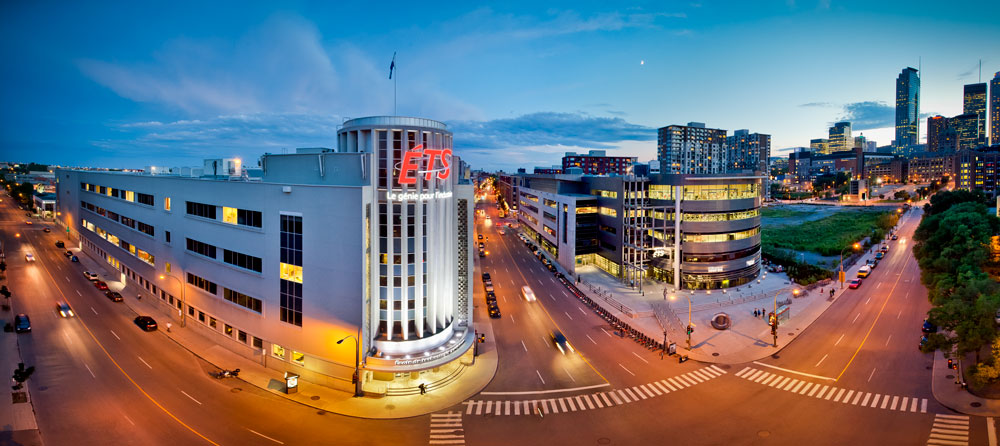
\includegraphics[width=0.75\textwidth]{Figures/vueEts.jpg} % Spécification du paramètres "width", la largeur de l'image (en conservant les proportions). La largeur est ici restreinte à 0.75 fois "\textwidth", qui est la largeur maximale du texte dans le document en prenant en compte les marges
	}
	 \\ \parbox{0.75\textwidth}{\caption{Test de longue légende, avec utilisation de framebox et parbox pour restreindre la largeur de la légende.}\label{fig:vueEts}} % Utilisation d'une parbox pour restreindre la largeur de la légende. Ici la taille maximale a été fixée à la largeur choisie pour l'image (0.75\textwidth). Le décanat demande d'éviter d'avoir des légendes qui dépasse les figures, dans la mesure du possible (si l'image est trop petite, la légende peut dépasser sa largeur).
\end{figure}

\lipsum[1] % Texte de remplissage pour donner un exemple de la mise en page


\end{introduction}

%%- Décommenter pour section revue de littérature, pour les thèses par article -%%
%\begin{revuedelitterature}
%%
%\end{revuedelitterature}

\chapter{Problématique et contexte}

% Quel sont les problèmes généraux et spécifiques que vous cherchez à solutionner – totalement ou en
% partie? Quel est le contexte de ces problèmes? Quelle est la situation actuelle?

Ce projet s'intéresse à l'étude des systèmes de types dans le contexte des langages de
programmation. Voici une définition possible :

\begin{quotation} % Benjamin C. Pierce, Types and Programming Languages, §1.1
  Un système de type est une méthode syntaxique ???tractable??? pour prouver l'absence de certains
  comportement des programmes par la classification des phrases selon le genre de valeurs qu'elles
  calculent.
\end{quotation}

L'objectif d'un système de type est donc de garantir, sans exécution, qu'un programme est exempt de
certaines erreurs (e.g. l'utilisation de deux systèmes d'unité, sans effectuer les conversions
appropriées, qui a entrainé la destruction du Mars Climate Orbiter). Ainsi, il existe un très grand
nombre de systèmes de types de divers niveau d'expressivité et de complexité. Lors du développement
d'un système de type, un ensemble de preuves est réalisé afin de démontrer que le nouveau système
respecte ses objectifs.

L'étude de ces systèmes ainsi que des preuves qui les accompagnent sont le sujet du présent projet.

\chapter{Objectif du projet}

% Dans cette partie, vous décrivez précisément  ce que vous allez accomplir dans le projet. Quels
% sont les résultats attendus de votre projet? Quelles sont les retombées du projet? Assurez-vous
% que vos objectifs sont "testables", c'est-à-dire que vous serez capable de démontrer de façon
% convaincante, à la fin du projet, que les objectifs ont été atteints. Assurez-vous aussi que vos
% objectifs sont en lien avec la problématique énoncée plus haut.

% Learning (Paper-Proof of Type Systems properties & Isabelle/HOL)
% Validate Paper-Proofs
% Clarification (Paper-Proof & Isabelle/HOL)

Les objectifs de ce projet sont quadruples : s'initier à la formalisation avec l'assistant de preuve
Isabelle/HOL, s'initier à la théorie des types, valider les preuves manuelles existantes et
clarifier les cas limites de ces dernières.

Isabelle/HOL est un assistant de preuve utilisant la logique d'ordre supérieure. Il permet de
spécifier des formules mathématiques, relations et algorithmes, de prouver des propriétés de ces
derniers et de générer du code exécutable correspondant à ces spécification. Ce projet se
concentrera sur la spécification de systèmes de types et l'écriture de preuves des différentes
propriétés qui y sont associées.

La théorie des types est un domaine d'étude à l'intersection de la logique, des mathématiques et de
la philosophie. Son application à l'informatique permet de vérifier, sans exécution, qu'un programe
respecte certaines propriétées. Les languages de programmtions dominants actuellement ne fournissent
qu'un nombre limité de garanties. Cependant, des alternatives plus expressives et plus puissantes
sont connues ou bien en développement.

La théorie des types étant un sujet de recherche très actif depuis plusieur dizaines d'années, un
grand nombre de publications décrivent les caractéristiques de différents systèmes de type.
Cependant, une formalisation manuelle étant valider par des être humains, il est toujours possible
que des erreurs s'y soient glissées. La formalisation de celles-ci à l'aide d'un assistant de preuve
permet de valider, sous réserve de l'assistant de preuve est correct, qu'aucune erreur logique n'est
présente.

Les propriétés énoncées et prouvées manuellement semblent souvent évidentes dès lors qu'elles sont
appliquées à un exemple concret. Cette méthode de visualisation a toutefois ses limites puisque
certaines constructions plus complexes peuvent entrainer des résultats inattendus. La formalisation
de ces propriétés à l'aide d'un assistant de preuve oblige son auteur à considérer la liste
exhaustive des constructions du language et permet ainsi d'acquérir un meilleur compréhension de la
propriété et des cas limites.

\chapter{Méthodologie}

% Expliquez comment vous allez atteindre les objectifs du projet. Ce sont les activités (analyse,
% conception, mesure, tests, gestion de la configuration, revues, etc.) et les responsabilités
% identifiées dans cette section qui guideront l’affectation des responsabilités aux membres de
% l’équipe et aussi à l’établissement de votre échéancier de travail.
%
% Note : une approche itérative est recommandée.

L'ouvrage de référence de ce projet est le livre « Types and Programming Languages » de Benjamin c.
Pierce. Ce livre est composé de six sections : les systèmes non-typés, les types simples, le
sous-typage, les types récursifs, le polymorphisme et les systèmes d'ordre supérieur. Chaque section
est composé de plusieurs chapitres décrivant un système de type bonifiant les systèmes décrits
précédemments en leur adjoignant un concept supplémentaire. Les figures \ref{fig:TAPL-section-1} et
\ref{fig:TAPL-section-2} présentent les chapitres des deux premières sections\footnote{Les chapitres
en gras sont ceux qui seront formalisés.} sur lesquelles se concentrera ce projet.

\todo[noline]{Trouver pourquoi le \\begin\{center\} ne fonctionne pas.}

\begin{figure}
  \begin{center}
    \begin{enumerate}[label=§\arabic*]
        \setcounter{enumi}{2}
      \item \textbf{Expressions arithmétiques non-typées}
      \item Une implémentation en ML des expressions arithmétiques
      \item \textbf{Le lambda-calcul non-typé}
      \item Représentation non-nommé des termes
      \item Une implémentation en ML du lambda-calcul
    \end{enumerate}
  \end{center}
  \caption{Section I du livre de référence --- Les systèmes non-typés}
  \label{fig:TAPL-section-1}
\end{figure}

\begin{figure}
  \begin{center}
    \begin{enumerate}[label=§\arabic*]
        \setcounter{enumi}{7}
      \item \textbf{Expressions arithmétiques typées}
      \item \textbf{Le lambda-calcul simplement typé}
      \item Une implémentation en ML des types simples
      \item Extensions simples
      \item Normalisation
      \item Références
      \item Exceptions
    \end{enumerate}
  \end{center}
  \caption{Section II du livre de référence --- Les types simples}
  \label{fig:TAPL-section-2}
\end{figure}

Le projet formalisera donc séquentiellement les différents chapitres en se basant, au besoin, sur le
travail fait pour les chapitres précédents. Chacune des formalisations se fera en quatre étapes :

\begin{enumerate}
  \item Lecture attentive du chapitre et compréhension générale des concepts énoncés;
  \item Définition dans Isabelle/HOL des structures nécessaires à la formalisation;
  \item Preuve des différents exercices, lemmes et théorèmes avancés;
  \item Simplification des définitions et preuves.
\end{enumerate}

\chapter{Composition de l'équipe et rôles}

Confirmer avec monsieur Labbé que cette section n'est pas applicable.

\chapter{Livrables et planification}

\section{Description des artéfacts}

% Cette section identifie les artefacts qui seront produits durant le projet, ainsi que la
% planification de leur réalisation.

\section{Planification}

% Voir Annexe A. Commentez le tableau de l’annexe A. Une approche itérative est recommandée.

\chapter{Risques}

% Vous devez énumérer les difficultés probables que vous pourriez rencontrer et qui pourraient avoir
% un impact sur la réalisation de votre projet. Vous devez expliquer dans un tableau chaque risque
% identifié, son impact ainsi que les moyens que vous allez mettre en œuvre pour le gérer et
% atténuer sa probabilité ou son impact.

% La forme d'un risque devrait être négative. C'est-à-dire, un risque est un événement que l'on veut
% éviter. Par exemple "expérience du client" n'est pas un risque tandis que "manque d’expérience du
% client" en serait un. Voici un exemple de risque : "Un passager est blessé dans une voiture lors
% d'une collision." Une mitigation à un risque est la stratégie qui vise à éviter que l'événement
% négatif se produise. Par exemple : "Le passager porte une ceinture de sécurité et la voiture est
% équipée de coussin de sécurité gonflable." Soyez spécifique à votre projet. "Manque de temps pour
% finir le projet" et "Portée trop ambitieuse" sont des risques pour n'importe quel projet. Il n’est
% pas mauvais d’avoir des risques génériques, mais il est important d’aussi trouver plusieurs
% risques spécifiques à votre projet, de même que de trouver des mitigations qui sont spécifiques à
% votre projet.

% Si vous manquez d'inspiration, vous pouvez consulter la liste LOG_GTI_792_Generic Software Risk
% Factors.xls, disponible sur le site Web du cours sous la rubrique ‘Gabarits et guides’. Toutefois,
% faire attention de ne pas ainsi identifier des risques et mitigations qui sont applicables à la
% majorité des projets.

\begin{table}
  \caption{Risques et mitigation}
  \begin{tabular}{|l|l|l|l|}
    \hline
    {\bf Risque} & {\bf Impact} & {\bf Probabilité} & {\bf Mitigation/atténuation} \\
    \hline
    Design Difficulty & & & \\
    \hline
    Implementation Difficulty & & & \\
    \hline
    Project Management Experience & & & \\
    \hline
    Application Experience & & & \\
    \hline
    Software Experience & & & \\
    \hline
  \end{tabular}
\end{table}

\chapter{Techniques et outils}

\todo[noline]{Ajouter une référence vers les différentes documentations des outils.}

\begin{description}
  \item[Isabelle] Système générique pour l'implémentation de formalismes logiques.
  \item[Isabelle/HOL] Spécialisation d'Isabelle pour la logique d'ordre supérieur (\gls{HOL}).
  \item[Isabelle/Isar] Language structuré permettant d'écrire des preuves plus lisibles.
  \item[Isabelle/jEdit] Environement de développement Isabelle basé sur jEdit.
  \item[Sledgehammer] Outils appliquant des prouveurs de théorèmes automatiques ainsi que des
    solveurs de « satisfaisabilité modulo théories »
\end{description}

\chapter{Références}

% \begin{equation}
%    \bm{\gamma} = \alpha \times 3
% \end{equation}


%Citation d'une référence de la bibliographie \cite{Arica2002}.
%Citation d'une référence de la liste de référence "refs" déclarée au début du document \citerefs{Test}.
%Référence à une Figure associée à un label: Figure \ref{fig:vueEts}.
%\href{http://www.etsmtl.ca/Etudiants-actuels/Cycles-sup/Realisation-etudes/Guides-gabarits}{Lien vers la page des gabarits de l'ÉTS}.
%\url{http://www.etsmtl.ca/Etudiants-actuels/Cycles-sup/Realisation-etudes/Guides-gabarits}.

\begin{conclusion}

\lipsum[1] % Texte de remplissage pour donner un exemple de la mise en page

\end{conclusion}


%%%%%%%%%%%%%%%%%%%%%%%%%%%%%%%%%%%%%%%%%%%%%%%%%%%
%  EXEMPLE D'ANNEXE:
%%%%%%%%%%%%%%%%%%%%%%%%%%%%%%%%%%%%%%%%%%%%%%%%%%%
\appendix

%% Lorsqu'on a plus qu'une annexe.
\multiannexe

%% Inclusion d'une annexe externe
% \include{extAnnex}

\chapter{Test d'une annexe}


\section{Première Section de l'Annexe}


\subsection{Figures en annexe}

\begin{figure}
	\centering
	\fbox{
		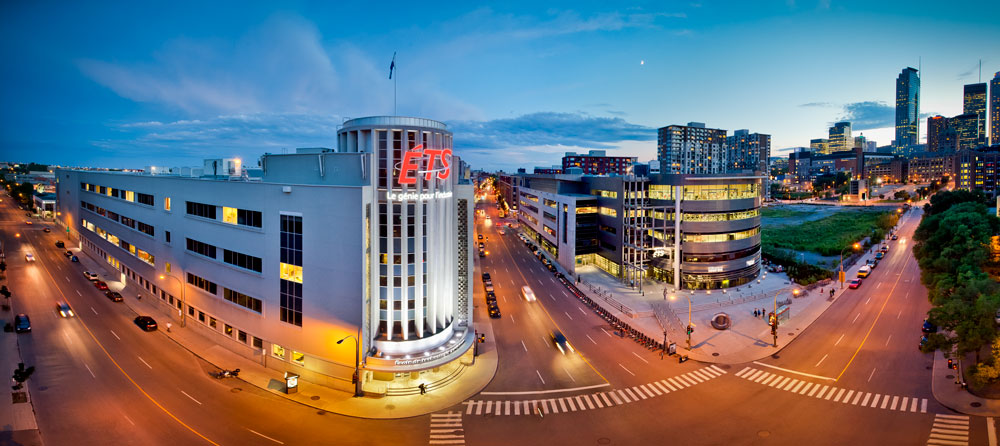
\includegraphics[width=0.75\textwidth]{Figures/vueEts.jpg}
	}
	 \\ \parbox{0.75\textwidth}{\caption{Figure en Annexe.}\label{fig:testAp}}
\end{figure}

Les figures en annexe se déclarent de la même manière que dans le reste du document, et leur numération est automatiquement adaptée (exemple, Figure \ref{fig:testAp}).

\subsubsection{Tables en annexe}

\begin{table}
		\parbox{0.65\textwidth}{\caption{Table en Annexe.}\label{tab:testAp}}

		\begin{tabular}{|c|c|c|c|c|c|c|c|}
		\hline
			{\bf titre} & {\bf titre} & {\bf titre} & {\bf titre} & {\bf titre} & {\bf titre} & {\bf titre} & {\bf titre} \\
	  \hline
			blá & blá & blá & blá & blá & blá & blá & blá \\
	  \hline
			blá & blá & blá & blá & blá & blá & blá & blá \\
	  \hline
			blá & blá & blá & blá & blá & blá & blá & blá \\
	  \hline
			blá & blá & blá & blá & blá & blá & blá & blá \\
	  \hline
			blá & blá & blá & blá & blá & blá & blá & blá \\
	  \hline
			blá & blá & blá & blá & blá & blá & blá & blá \\
	  \hline
		\end{tabular}
\end{table}

Même chose pour les tableaux (exemple, Tableau \ref{tab:testAp}).


%%%%%%%%%%%%%%%%%%%%%%%%%%%%%%%%%%%%%%%%%%%%%%%%%%%
% BIBLIOGRAPHIE ET RÉFÉRENCES
%%%%%%%%%%%%%%%%%%%%%%%%%%%%%%%%%%%%%%%%%%%%%%%%%%%

%%- Bibliographie -%%
\newpage
%Interligne sinmple pour la bibliographie
\begin{spacing}{1}
	\nocite{*} % Utiliser la commande nocite pour afficher des références qui n'ont pas été citées dans le document. '*' permet de toutes les afficher.
	\bibliographystyle{bibETS} % Utilisation du style bibliographique de l'ETS
	\addcontentsline{toc}{chapter}{BIBLIOGRAPHIE} % Ajout de la bibliographie à la table des matières

	\bibliography{biblio} % Liste des fichiers bib de bibliographie, biblio.bib est un exemple

\end{spacing}

%%- Références, exemple des références "refs" --%
%%%%%%%%%%%%%%%%%%%%%%%%%%%%%%%%%%%%%%%%%%%%%%%%%%%
% IMPORTANT: NOTES POUR COMPILER ET AFFICHER LES RÉFÉRENCES ADDITIONNELLES (remplacer "refs" par le suffixe choisi)
%%%%%%%%%%%%%%%%%%%%%%%%%%%%%%%%%%%%%%%%%%%%%%%%%%%
% Suivre les trois étapes:
%   1. Compiler le document une fois pour renseigner les références utilisées dans refs.aux
%   2. Lancer la compilation des références
% 		- Sous Linux: Utilser la commande "bibtex refs" dans le dossier du document
%		- Sous MacOSX (distribution MacTex): Utilser la commande "/usr/texbin/bibtex refs" dans le dossier du document
%		- Sous Windows: Éditer le script "update_refs.bat" pour renseigner le bon suffixe, et le lancer
%   3. Recompiler le document deux fois
%%%%%%%%%%%%%%%%%%%%%%%%%%%%%%%%%%%%%%%%%%%%%%%%%%%

\newpage
% Le fonctionnement est similaire, en rajoutant le suffixe choisi "refs" à la fin de chaque commande de bibliographie
\begin{spacing}{1}
	%\nociterefs{*}
	\bibliographystylerefs{bibETS}
	\addcontentsline{toc}{chapter}{LISTE DE RÉFÉRENCES}

	\bibliographyrefs{refs} % Liste des fichiers bib de référence, refs.bib est un exemple

\end{spacing}

\end{document}
